

% Chapter 4 — Sprint 1 (Overleaf-ready)
% Compile with pdfLaTeX. To integrate into an existing report, copy the content
% from \setcounter{chapter}{3} onward and keep packages in your main preamble.
\documentclass[12pt,a4paper]{report}

\usepackage[utf8]{inputenc}
\usepackage[T1]{fontenc}
\usepackage[english]{babel}
\usepackage{geometry}
\geometry{margin=2.5cm}
\usepackage{graphicx}
\usepackage{array}
\usepackage{tabularx}
\usepackage{longtable}
\usepackage{booktabs}
\usepackage{float}
\usepackage{xcolor}
\usepackage{hyperref}
\usepackage{enumitem}
\usepackage{caption}
\usepackage{microtype}
\hypersetup{colorlinks=true,linkcolor=black,urlcolor=blue,citecolor=black}
\setlength{\parskip}{0.45em}
\setlength{\parindent}{0pt}
\renewcommand{\arraystretch}{1.18}
\newcolumntype{Y}{>{\raggedright\arraybackslash}X}

% Empty, clearly labeled space for a diagram that will be supplied later.
\newcommand{\diagramplaceholder}[2][6cm]{%
  \begin{figure}[H]
    \centering
    \fbox{\parbox[c][#1][c]{0.94\textwidth}{\centering\textit{Diagram to be inserted by the team}}}
    \caption{#2}
  \end{figure}%
}

% Empty space for implementation screenshots to be supplied later.
\newcommand{\screenshotplaceholder}[1]{%
  \begin{figure}[H]
    \centering
    \fbox{\parbox[c][5cm][c]{0.88\textwidth}{\centering\textit{Screenshot to be inserted by the team}}}
    \caption{#1}
  \end{figure}%
}

\begin{document}
\setcounter{chapter}{3}
\chapter{Sprint 1: Working Demo (Foundations, Rooms, and Ideation)}

\section{Introduction}


This chapter documents the sprint using the Scrum approach and the UML modeling principles established in Chapter 3. It presents the sprint organization and backlog (Section 4.2), the analysis through use cases (Section 4.3), the design through class, sequence, and activity diagrams (Section 4.4), the implementation and public demo setup (Section 4.5), and the sprint review and retrospective (Section 4.6).

The sprint contains 18 stories: four technical foundation tasks (T1--T4) and fourteen user stories covering authentication (US-1--US-4), rooms (US-9--US-12), ideas (US-22--US-25), and voting (US-35--US-36). All items are prioritized Must, for a total of 58 story points.

\section{Sprint 1 Organization}
\subsection{Sprint 1 Goal}
\textbf{Sprint goal:} Deliver a publicly deployed working demo in which a user can register, create a brainstorming room, invite others, post ideas, and vote.

The delivered value is an end-to-end demo that can be presented to the academic supervisor and potential users. It demonstrates the complete application chain---frontend, backend, database, and deployment---and the core brainstorming loop: join a room, contribute ideas, and vote. Later sprints build on these foundations by adding real-time collaboration and AI features, followed by subscriptions and administration capabilities.

\subsection{Sprint 1 Backlog}
The backlog contains 18 Must-priority items. Story points follow the Fibonacci scale. The total sprint estimate is 58 story points.

\begingroup
\small
\renewcommand{\arraystretch}{1.35}
\setlength{\tabcolsep}{8pt}
\begin{longtable}{@{}p{0.075\textwidth}p{0.20\textwidth}p{0.075\textwidth}p{0.52\textwidth}p{0.07\textwidth}@{}}
\caption{Sprint 1 backlog}\label{tab:sprint1-backlog}\\
\toprule
\textbf{ID} & \textbf{Story} & \textbf{Priority} & \textbf{Technical tasks} & \textbf{Points} \\
\midrule
\endfirsthead
\toprule
\textbf{ID} & \textbf{Story} & \textbf{Priority} & \textbf{Technical tasks} & \textbf{Points} \\
\midrule
\endhead
\midrule
\multicolumn{5}{r}{Continued on next page}\\
\endfoot
\bottomrule
\endlastfoot
T1 & Repository, branching rules, automated build & Must & Create the shared repository; define branching and review rules; configure an automated build on every push. & 3 \\
T2 & Frontend, backend, and database connected end to end & Must & Scaffold the frontend and REST API; connect the API to the database; expose a health endpoint called by the frontend. & 5 \\
T3 & First schema and migrations & Must & Create the Sprint 1 data schema according to the class diagram (User, Client, Room, Idea, and Vote, with the depicted relationships); write versioned migrations; add seed data. & 3 \\
T4 & Public demo environment & Must & Provision hosting for frontend, API, and database; configure environment variables; deploy from the main branch. & 5 \\
US-1 & Register with name, email, and password & Must & Integrate user registration with Keycloak; validate the required fields and email uniqueness; link the application user to the Keycloak account. MindSpark does not store user passwords. & 5 \\
US-2 & Log in with email and password & Must & Authenticate credentials through Keycloak; use the returned bearer token for authenticated API requests; protect private routes by validating the token. & 3 \\
US-3 & Log out & Must & Implement the logout action and invalidate the client session. & 1 \\
US-4 & View my profile & Must & Provide an authenticated API endpoint that returns the signed-in user's profile data. & 2 \\
US-9 & Create a brainstorming room & Must & Build the room form with a title; generate a unique invitation code; set the creating user as owner. & 5 \\
US-10 & Join a room with an invitation code & Must & Build the join form; validate the code; create the participant record; handle invalid codes and duplicate joins. & 5 \\
US-11 & Leave a room & Must & Implement the leave action and remove the membership. If the room owner leaves, the room remains available, but the remaining participants can only leave the room; all other room actions are disabled. & 3 \\
US-12 & See my rooms and reopen them & Must & List rooms belonging to the user; build the My Rooms dashboard; open an existing room. & 3 \\
US-22 & Create an idea in my room & Must & Build the idea form; link each idea to its room and author; check room membership. & 3 \\
US-23 & Edit my own ideas & Must & Implement the edit action and verify that the requesting user is the author. & 2 \\
US-24 & Delete my own ideas & Must & Implement deletion with confirmation and verify that the requesting user is the author. & 2 \\
US-25 & View all participants' ideas & Must & List the ideas in a room with their authors and display them on the room canvas. & 3 \\
US-35 & Vote for an idea & Must & Implement voting; enforce at most one vote per user per idea; display vote counters. A user may vote for multiple different ideas. & 3 \\
US-36 & Remove my vote & Must & Allow a user to remove their vote and update the corresponding vote counter. & 2 \\
\midrule
\multicolumn{4}{r}{\textbf{Total}} & \textbf{58} \\
\end{longtable}
\normalsize

\section{Sprint 1 Analysis}
\subsection{Sprint 1 Use Case Diagrams}

The Sprint 1 use case analysis is divided into five diagrams: Authentication, Idea Management, Room Management, Vote Management, and Workspace Management. The main actor is the \textit{User}; depending on the use case, the user may act as a room owner or a participant.

\subsubsection{Authentication Use Case Diagram}

This diagram presents the actions a user can perform to access and manage an account, including registration, login, and  logout.

\begin{figure}[H]
    \centering
    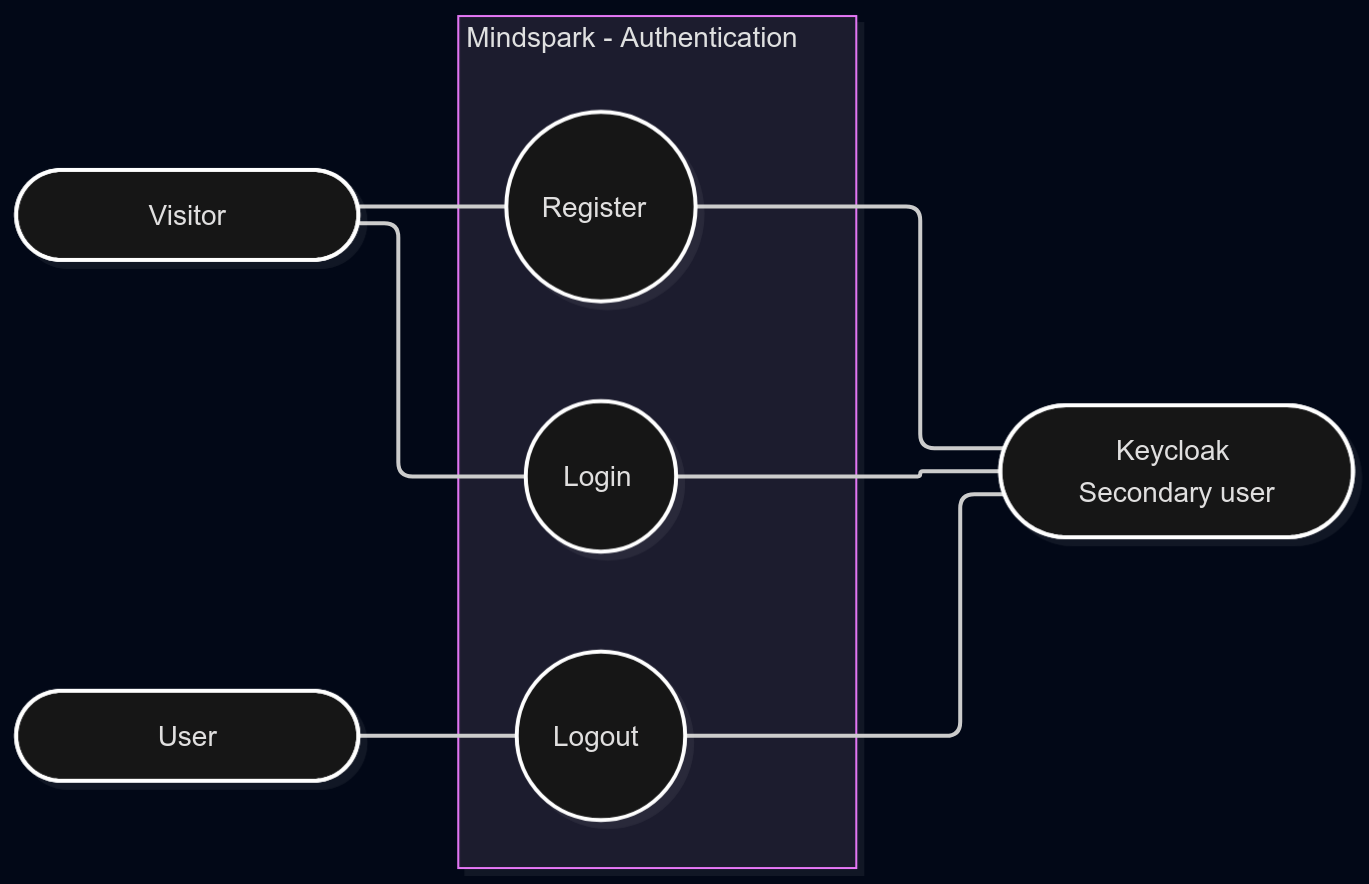
\includegraphics[width=0.85\textwidth]{authentification.png}
    \caption{Authentication use case diagram.}
    \label{fig:authentification.png}
\end{figure}

\subsubsection{Idea Management Use Case Diagram}

This diagram describes how a room participant interacts with ideas: creating an idea, viewing ideas in the room, editing their own ideas, and deleting their own ideas.


\begin{figure}[H]
    \centering
    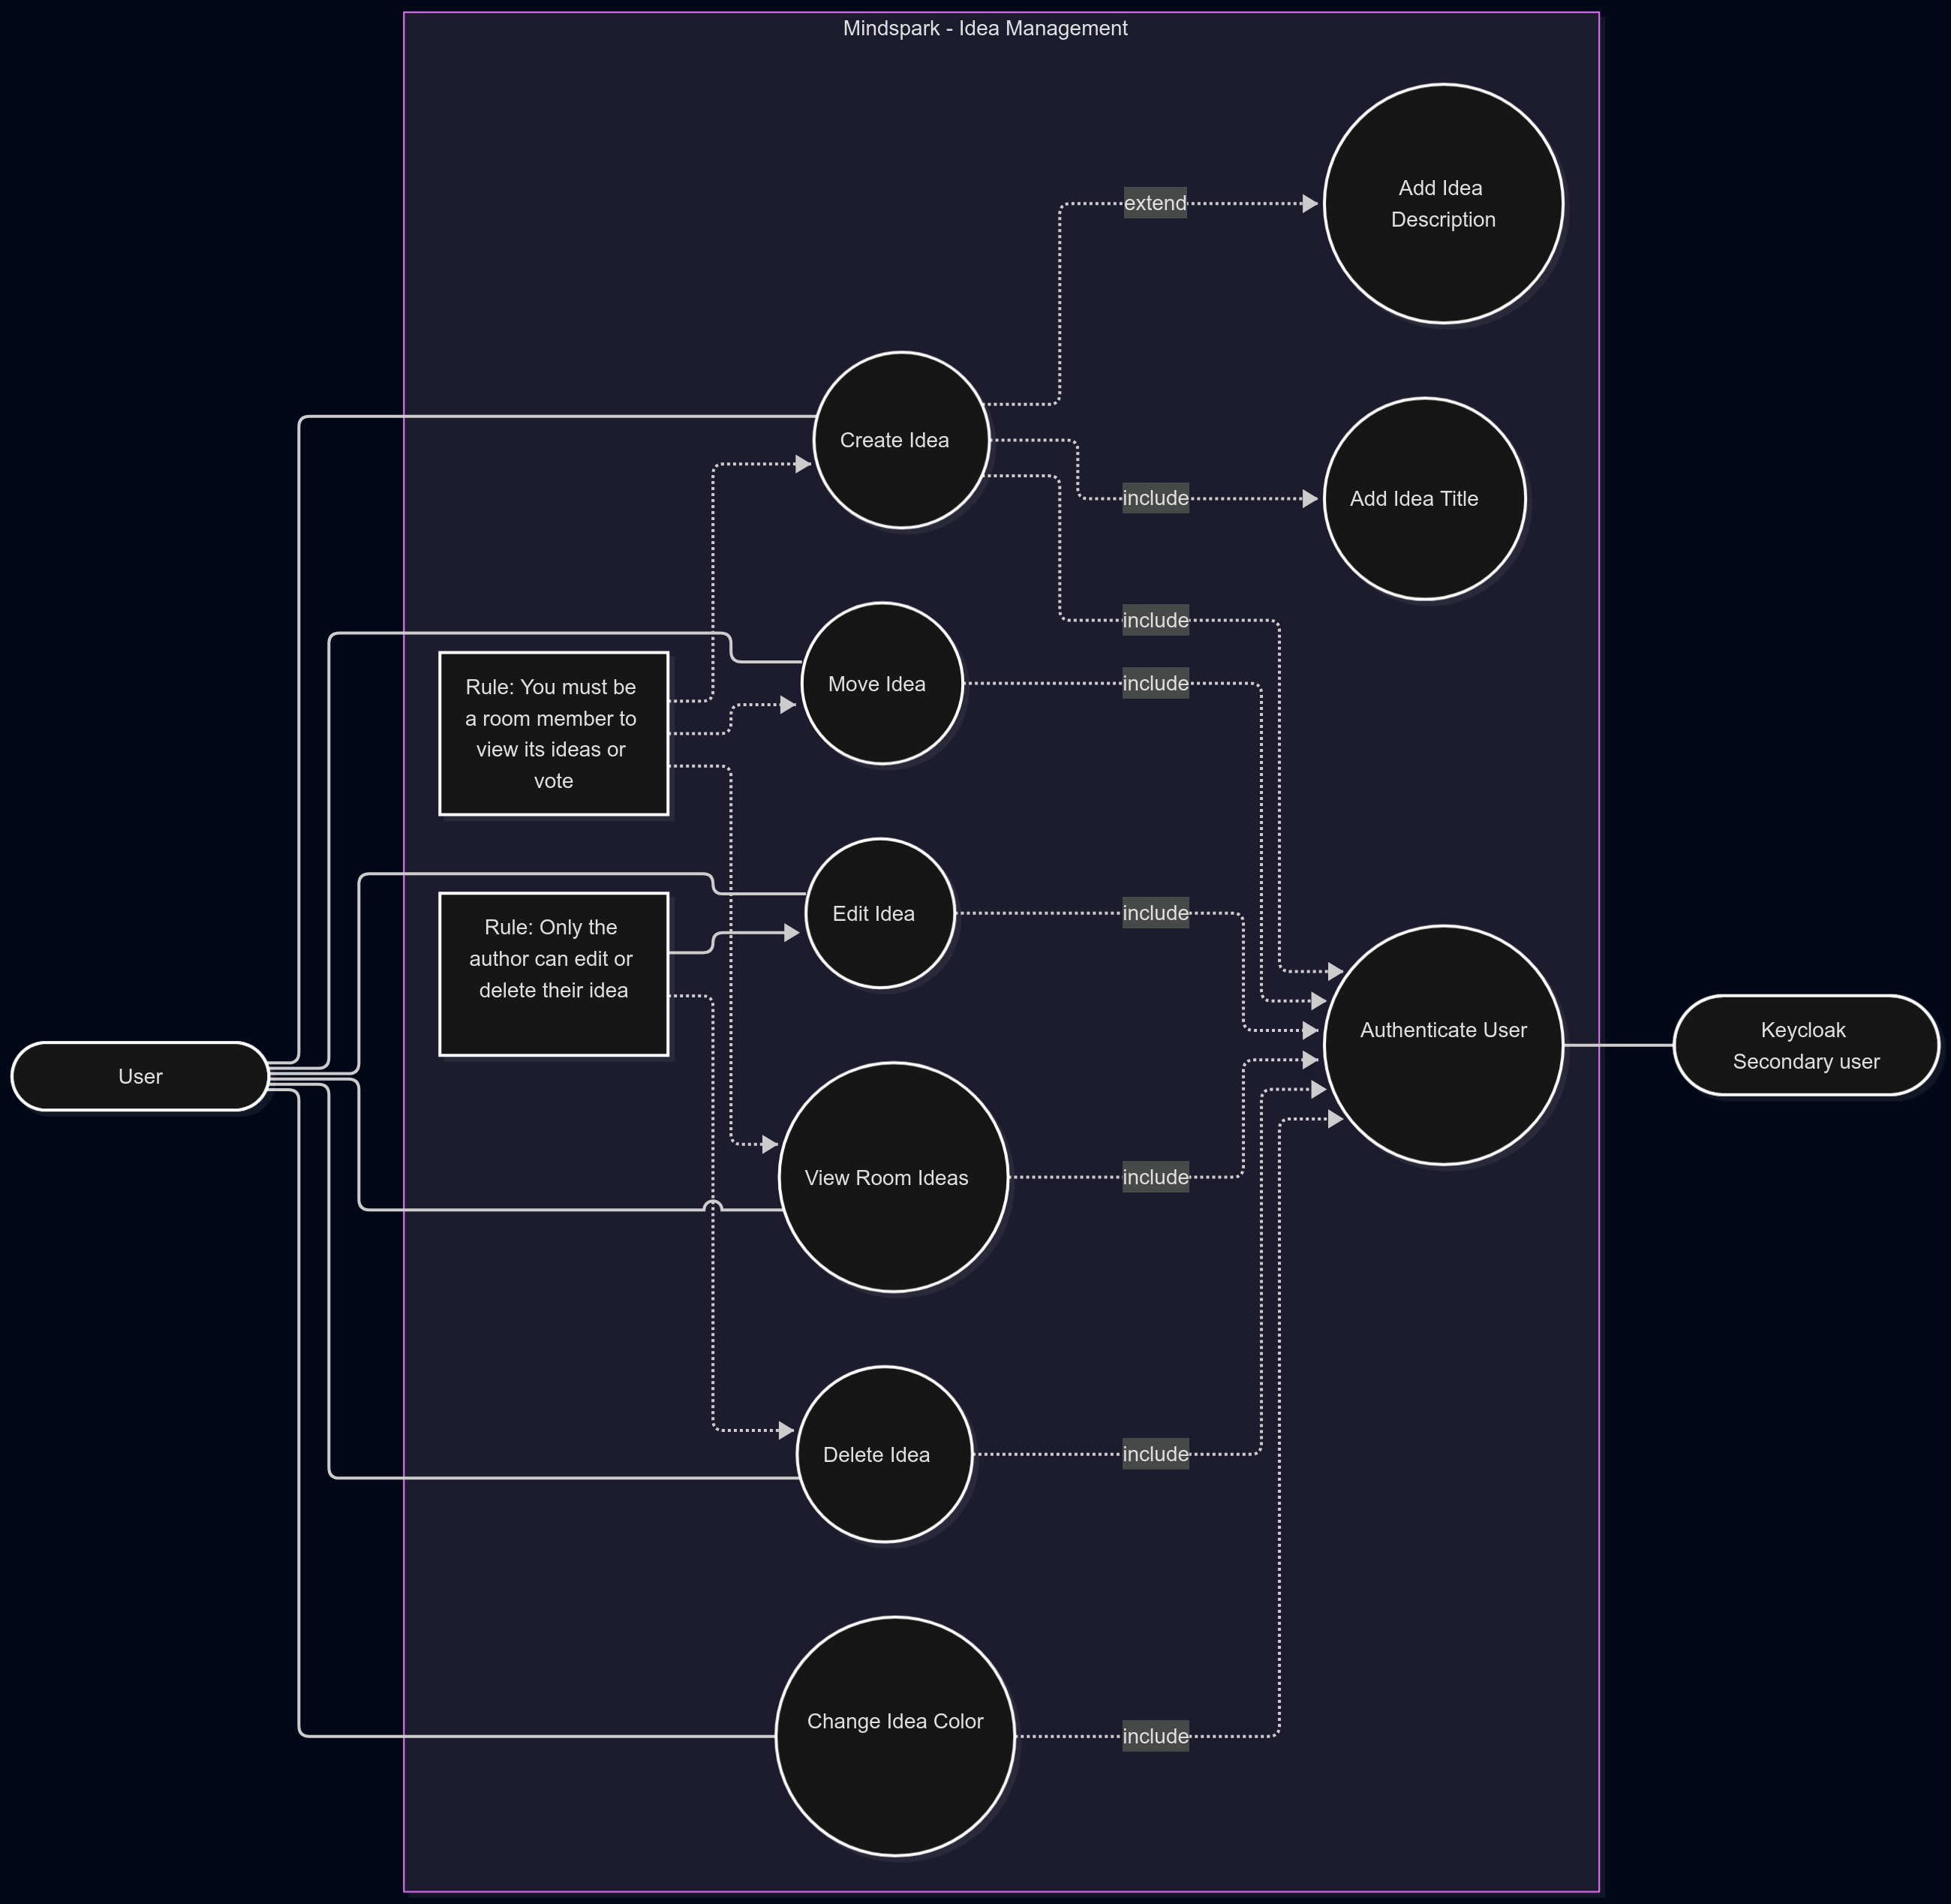
\includegraphics[width=0.85\textwidth]{idea management.png}
    \caption{idea-management-use-case.}
    \label{fig:idea-management-use-case}
\end{figure}

\subsubsection{Room Management Use Case Diagram}

This diagram covers creating a room, receiving  its invitation code, joining with a code, viewing or reopening rooms, and leaving a room. If the room owner leaves, the room remains, but the other participants can only leave; all other room actions are disabled for them.

\begin{figure}[H]
    \centering
    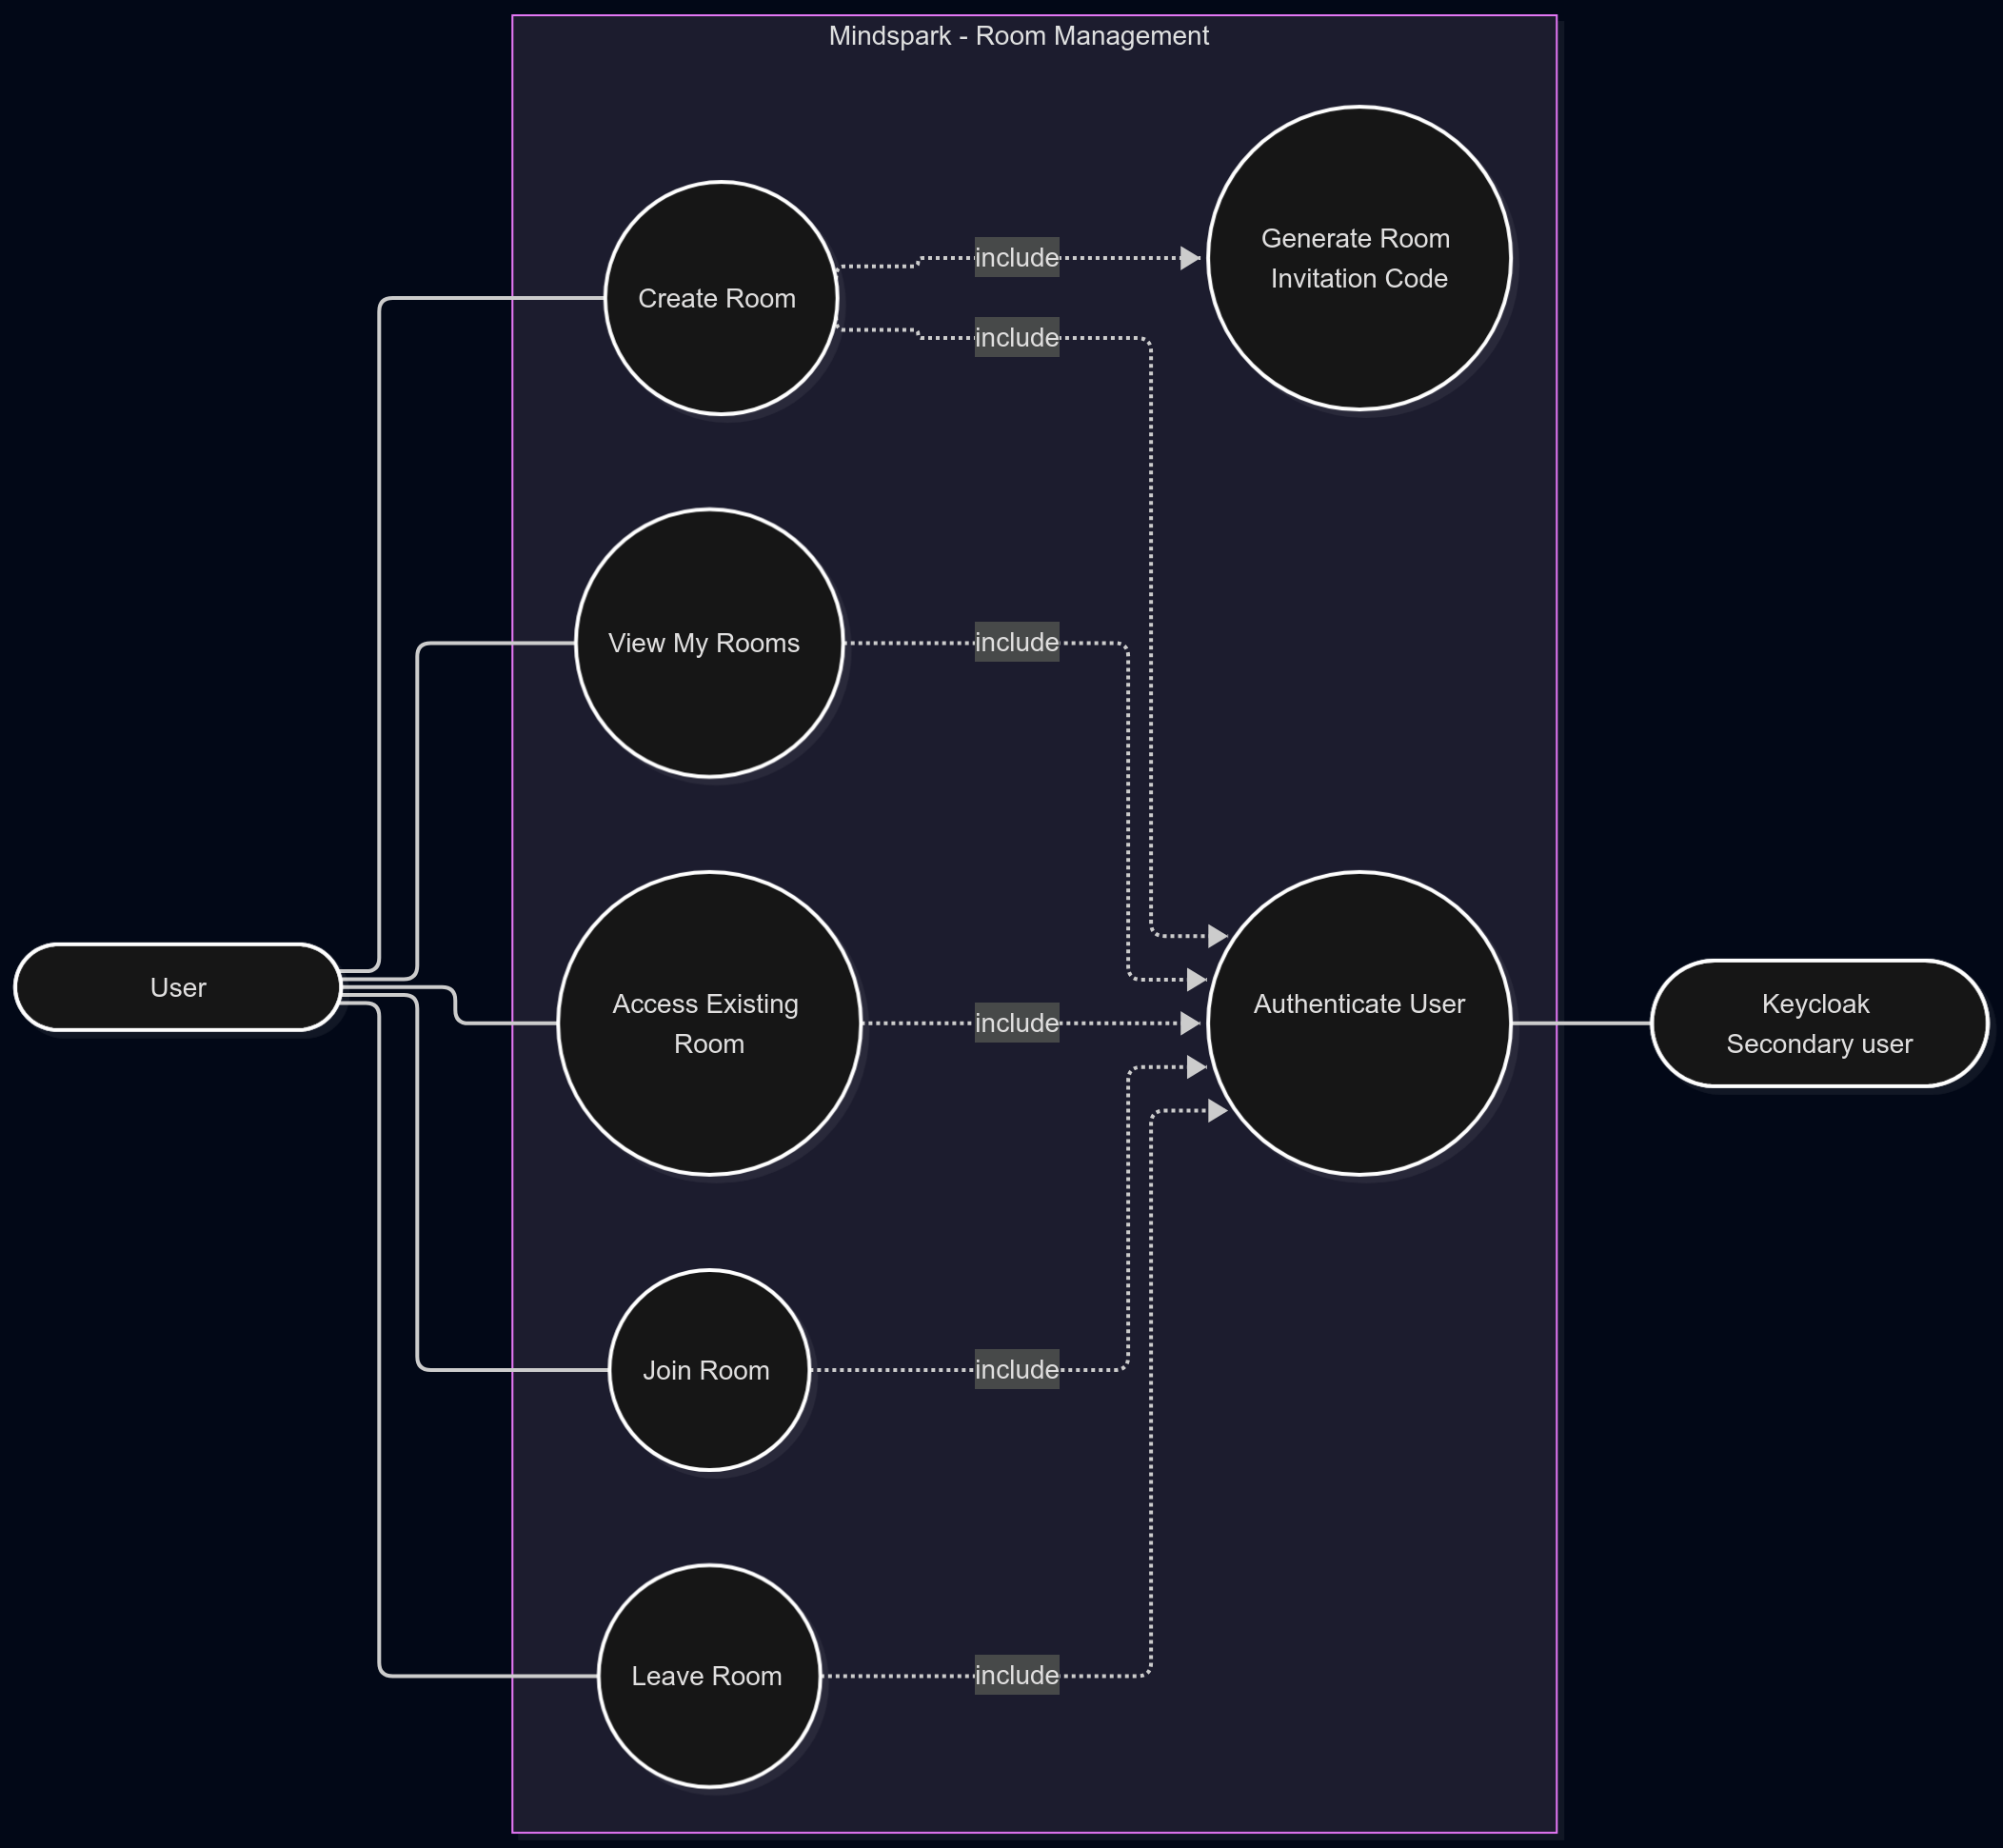
\includegraphics[width=0.85\textwidth]{room managment.png}
    \caption{room-management-use-case.}
    \label{fig:room-management-use-case}
\end{figure}


\subsubsection{Vote Management Use Case Diagram}

This diagram shows how a participant votes for an idea or removes a vote,. A user may vote for multiple ideas, but can have at most one vote on any individual idea.


\begin{figure}[H]
    \centering
    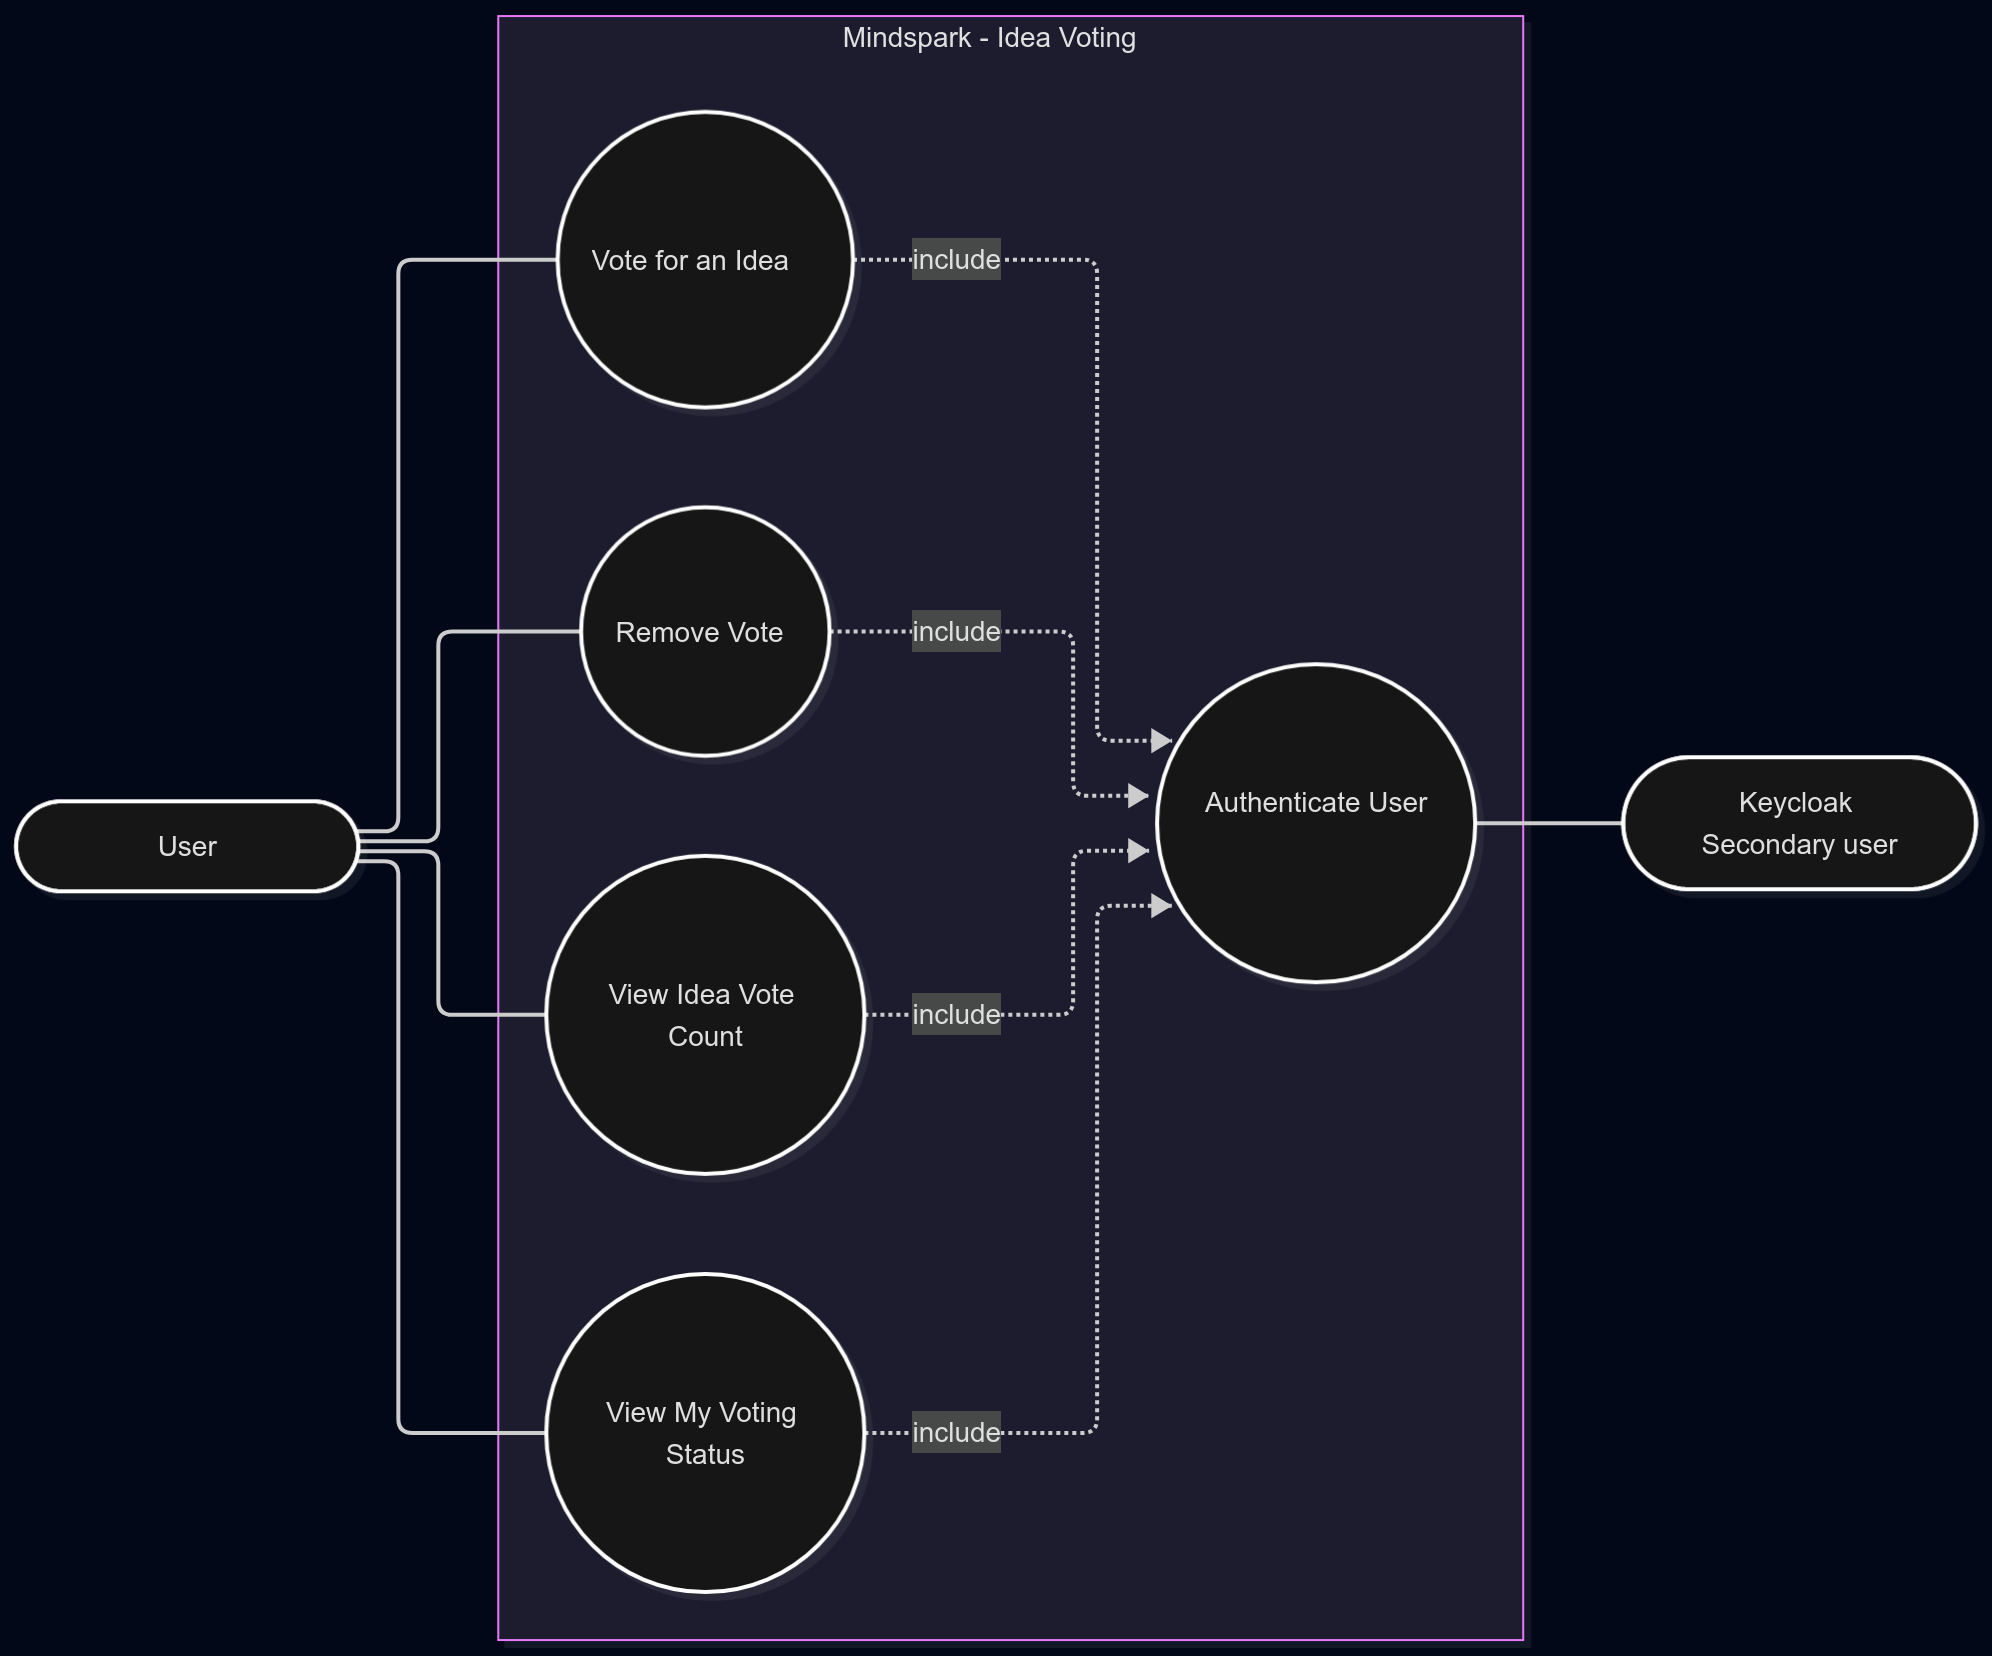
\includegraphics[width=0.85\textwidth]{vote management.png}
    \caption{vote-management-use-case.}
    \label{fig:vote-management-use-case}
\end{figure}

\subsubsection{Workspace Management Use Case Diagram}

This diagram represents the user's interaction with the brainstorming workspace and its available design tools, such as the eraser.

\begin{figure}[H]
    \centering
    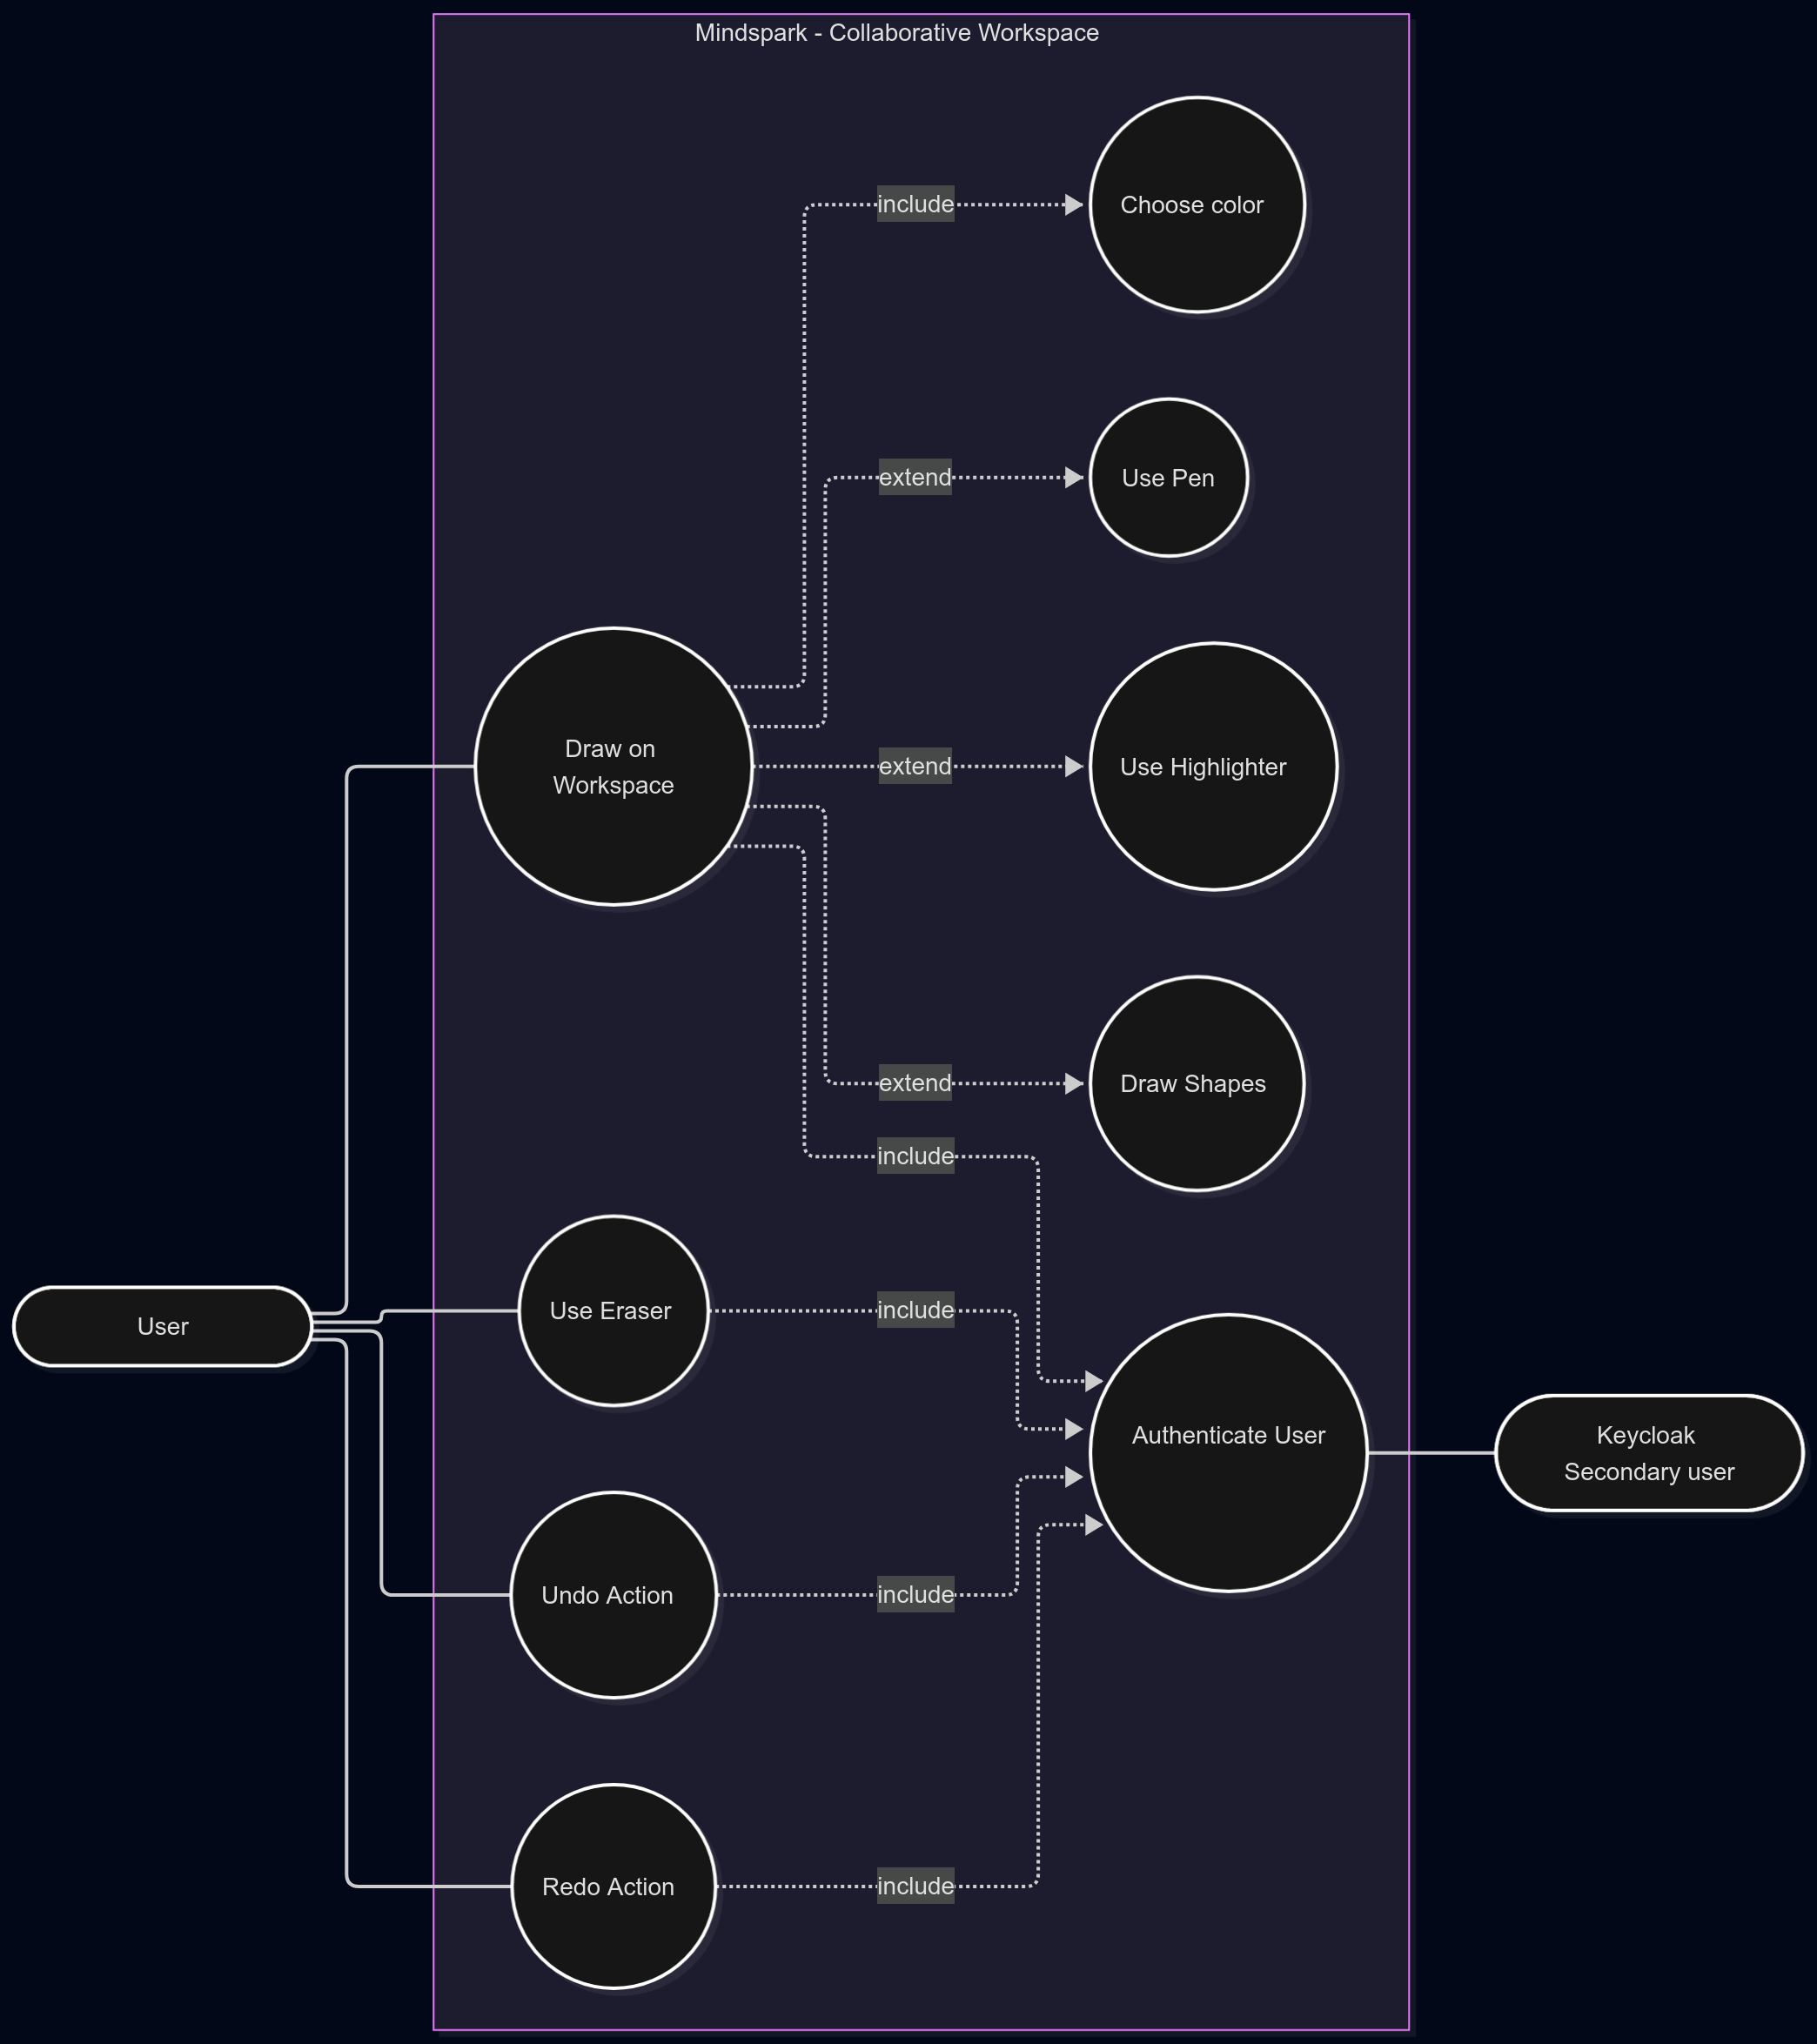
\includegraphics[width=0.85\textwidth]{workspace.png}
    \caption{workspace-management-use-case.}
    \label{fig:workspace-management-use-case}
\end{figure}

\subsection{Textual Use Case Descriptions}

\subsubsection{UC1 --- Create and Join a Brainstorming Room via Invitation Code (US-9, US-10)}
\begin{tabularx}{\textwidth}{|p{0.21\textwidth}|Y|}\hline
\textbf{Field} & \textbf{Description} \\\hline
Actors & Room Creator; Participant. \\\hline
Preconditions &Room creation: The user is registered and logged in.

Room joining: The individual who wants to join is registered and logged in and has received an invitation code from the room owner. \\\hline
Postconditions & A room exists with a unique invitation code and its creator as owner. After successful joining, the participant is a member and can see the room . \\\hline
Nominal flow & (1) The creator opens the room form. (2) The creator enters the title and submits. (3) The system validates the room details, creates the room, generates a unique invitation code, and assigns the creator as the room owner. (4) The owner receives the invitation code and shares it with the individuals who want to join the room. (5) An invited user enters the code in the join form. (6) The system validates the code, creates the membership, and opens the room. \\\hline
Alternative flows & A1 --- Missing or invalid room data: the system shows field errors and creates no room. A2 --- Unknown invitation code: the system reports an invalid code and creates no membership. A3 --- The user is already a member: the system opens the room without creating a duplicate membership. A4 --- The creator has left the room: remaining participants cannot perform room actions; they may only leave the room. \\\hline
\end{tabularx}

\subsubsection{UC2 --- Create, Edit, and Delete an Idea (US-22--US-24)}
\begin{tabularx}{\textwidth}{|p{0.21\textwidth}|Y|}\hline
\textbf{Field} & \textbf{Description} \\\hline
Actors & Participant, including the Room Creator while they remain in the room. \\\hline
Preconditions & The user is logged in and is a member of the room. For editing or deleting, the user is the author of the idea. If the room creator has left the room, remaining participants may not create, edit, or delete ideas. \\\hline
Postconditions & The idea is created, updated, or removed, and the room's idea list reflects the resulting state. Any votes attached to a deleted idea are also removed . \\\hline
Nominal flow & (1) The participant opens the room. (2) The participant enters the idea text and submits it. (3) The system checks membership and saves the idea with its author and room. (4) To edit, the author opens the idea, changes the text, and saves; the system updates it. (5) To delete, the author selects delete and confirms; the system removes the idea and its associated votes. \\\hline
Alternative flows & A1 --- Empty idea text: the system rejects the submission or edit and displays an error. A2 --- The user is not the author: the system denies the edit or deletion. A3 --- The author cancels deletion: the idea remains. A4 --- The room owner has left: The system disables all room actions for the remaining participants except leaving the room. \\\hline
\end{tabularx}

\subsubsection{UC3 --- Vote for an Idea and Remove a Vote (US-35, US-36)}
\begin{tabularx}{\textwidth}{|p{0.21\textwidth}|Y|}\hline
\textbf{Field} & \textbf{Description} \\\hline
Actors & Participant, including the Room Creator while they remain in the room. \\\hline
Preconditions & The user is logged in, is a member of the room, and the idea exists in that room. A user may vote for multiple different ideas, but may cast at most one vote for any particular idea. \\\hline
Postconditions & A vote is recorded or removed, and the corresponding vote counter is updated. \\\hline
Nominal flow & (1) The participant selects the vote action for an idea. (2) The system checks whether the user has already voted for that idea. If not, it records the vote and increments the counter. (3) The user may vote for other ideas, but may vote only once for each individual idea. (4) The participant selects the vote action again to remove their vote; the system deletes it and decrements the counter. \\\hline
Alternative flows & A1 --- The user has already voted for the idea: selecting the vote action removes the existing vote and updates the counter. A2 --- The idea no longer exists: the system refuses the vote and refreshes the idea list. A3 --- The room owner has left: the system disables all room actions for the remaining participants except leaving the room. \\\hline
\end{tabularx}

\section{Sprint 1 Design}
The class diagram presents the main structure of the MindSpark system. A visitor can register or log in, after which the system creates or accesses a \textit{User} account. User authentication is handled by Keycloak, and each user's email address must be unique.

The \textit{Client} class inherits from \textit{User} and represents an authenticated user interacting with the application. A client can view and reopen rooms, create or join a room using an invitation code, leave a room, and manage ideas and votes.

A client can create multiple rooms, while each room has one creator. A room has a unique invitation code and contains zero or more ideas. Each idea belongs to one room and is written by one client. Clients can cast votes on ideas; each vote is associated with one idea and one client. The model allows a client to vote for multiple ideas, while enforcing at most one vote per client for each idea.

Ideas include text, title, description, position, color, and creation and update timestamps. Only the author of an idea may edit or delete it, and the author must be a member of the room. The diagram also shows operations for creating, updating, moving, and deleting ideas, as well as adding and removing votes.

\begin{figure}[H]
    \centering
    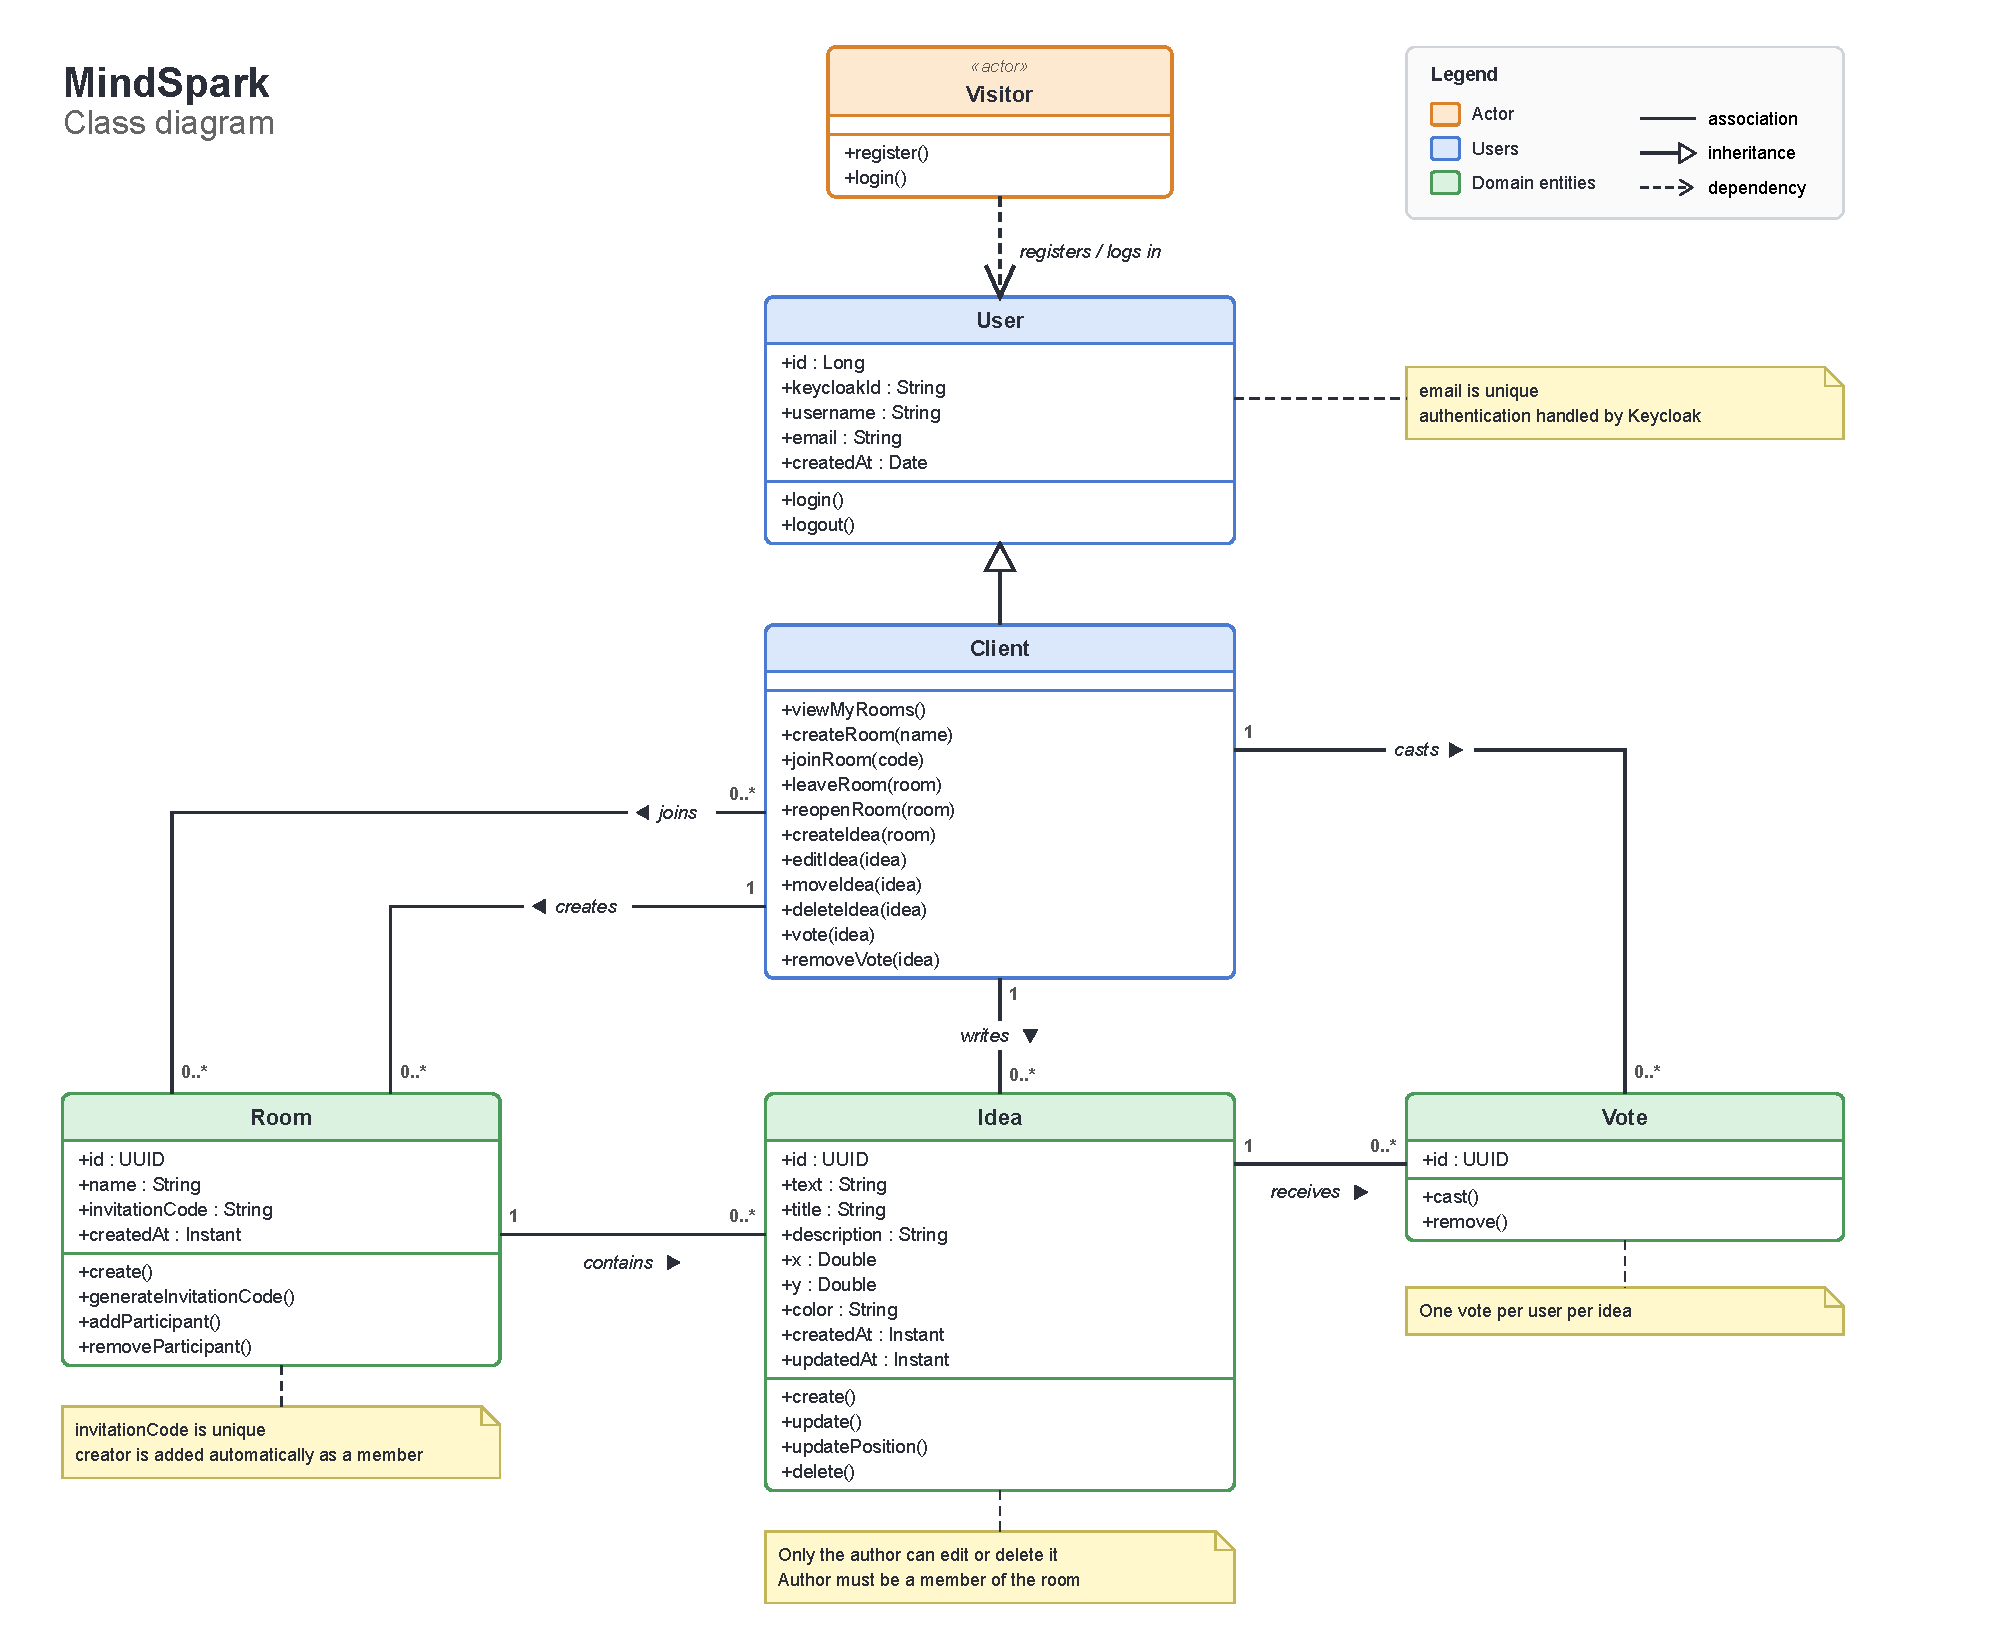
\includegraphics[width=\textwidth]{MindSpark class diagram.pdf}
    \caption{MindSpark class diagram}
    \label{fig:mindspark-class-diagram}
\end{figure}

\subsection{Design Sequence Diagrams}

The sequence diagrams describe the interactions between the user and the MindSpark system. The original diagram is divided into three functional areas: authentication, room management, and idea and vote management.

\subsubsection{Authentication Sequence Diagram}

This sequence diagram shows the registration and login requests sent by the user to the MindSpark system. The system returns the user information after a successful request. If the authentication token is missing or rejected, the system returns an unauthorized response. Authentication is handled by Keycloak, and authenticated API requests use a Keycloak bearer token.

\begin{figure}[H]
    \centering
    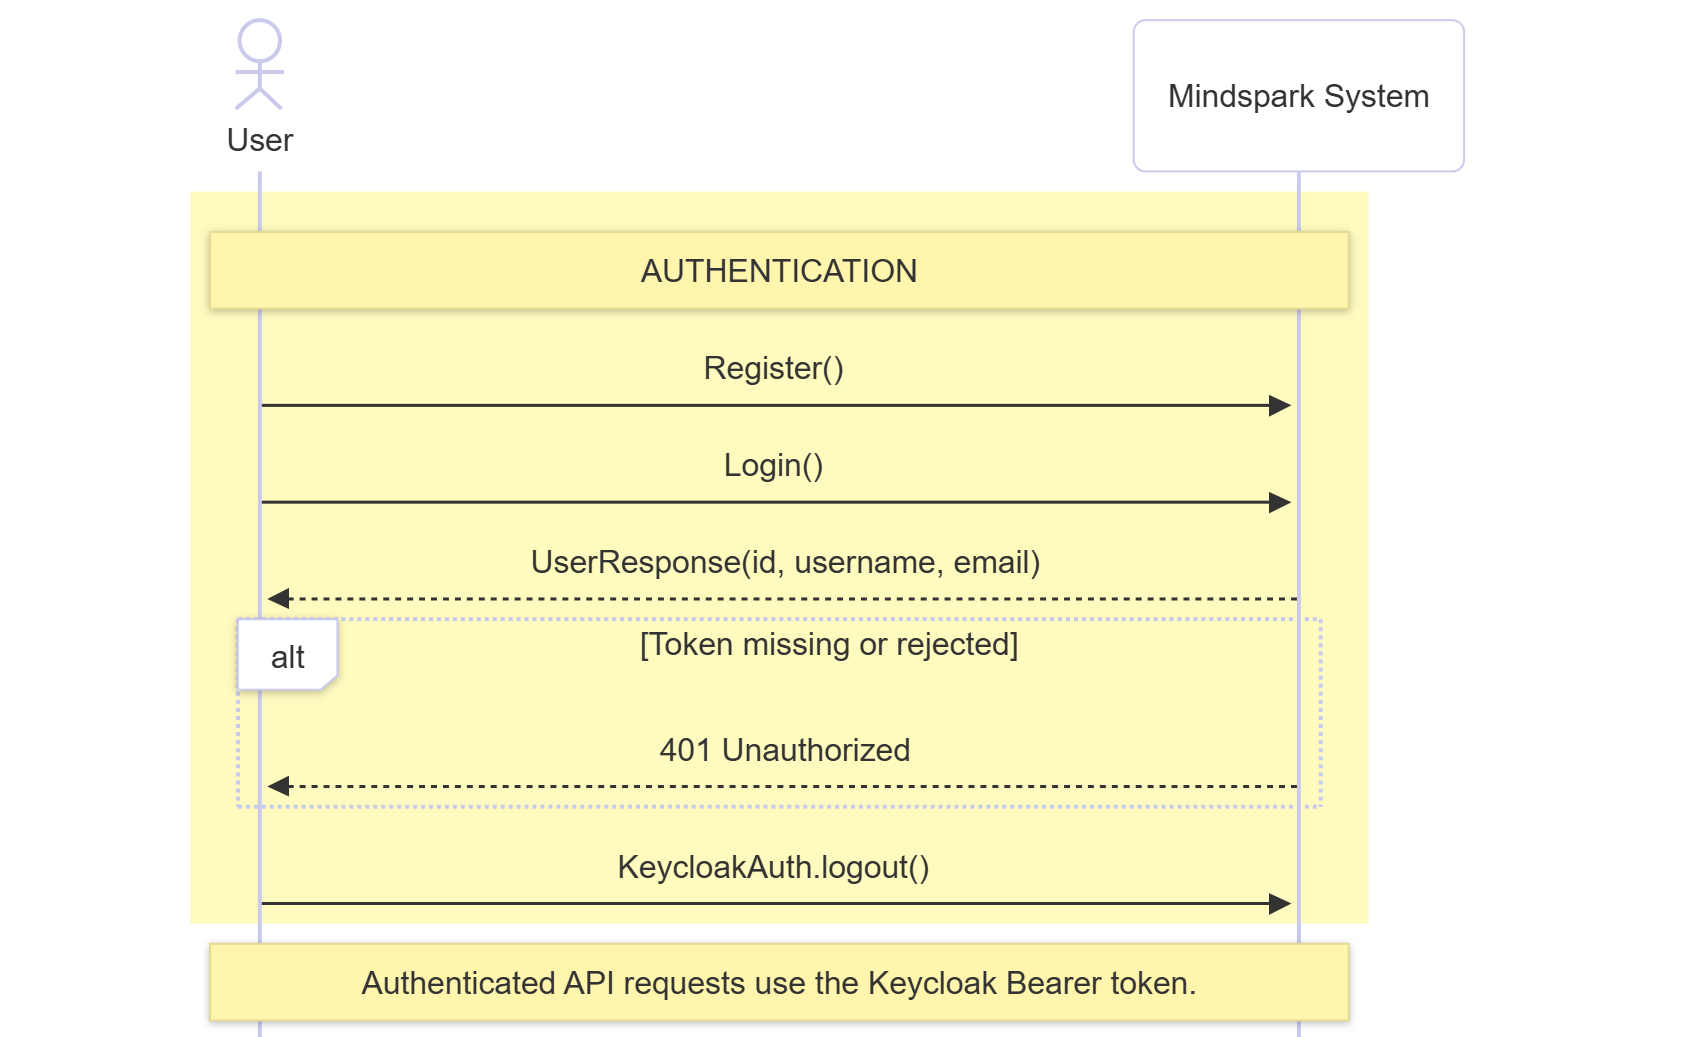
\includegraphics[width=0.95\textwidth,height=0.72\textheight,keepaspectratio]{Auth.png}
    \caption{Authentication sequence diagram}
    \label{fig:sequence-authentication}
\end{figure}

\subsubsection{Room Management Sequence Diagram}

This sequence diagram shows how a user creates a room, receives its invitation code, joins a room with that code, lists their rooms, reopens a room, and leaves it. The system checks the invitation code and the user's room membership. An invalid invitation code returns a not-found response, while a user who is not a room member is denied access. 

\begin{figure}[H]
    \centering
    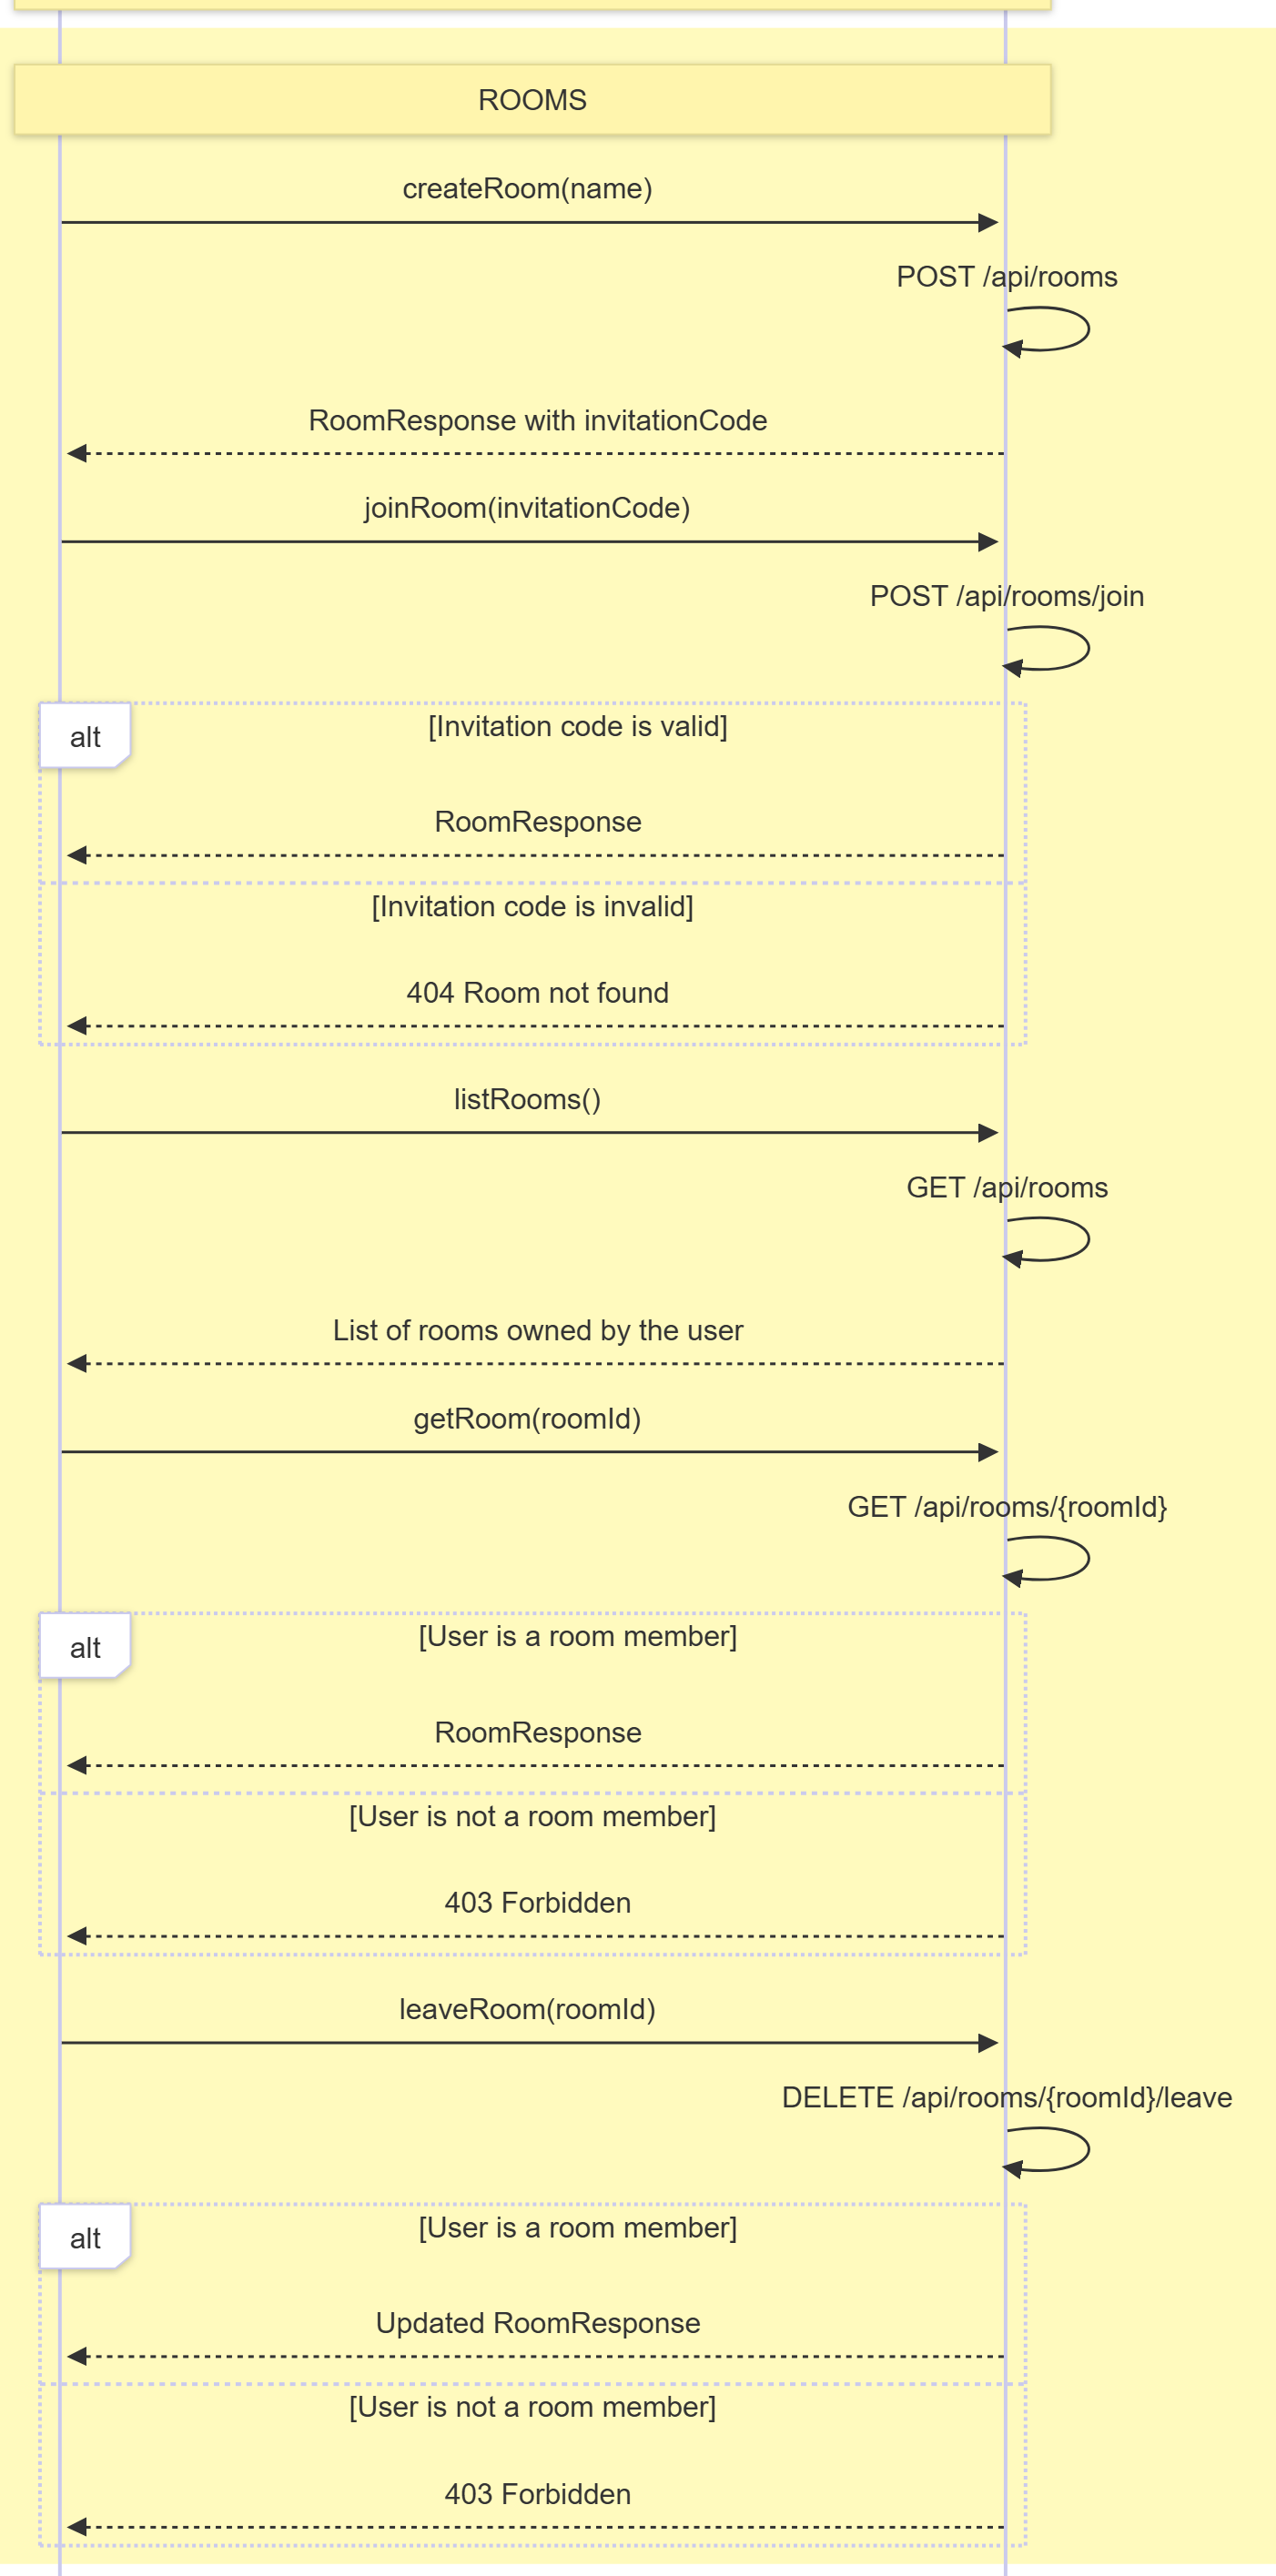
\includegraphics[width=0.95\textwidth,height=0.72\textheight,keepaspectratio]{Roomsdiag.png}
    \caption{Room management sequence diagram}
    \label{fig:sequence-room-management}
\end{figure}

\subsubsection{Idea and Vote Management Sequence Diagram}

This sequence diagram presents the operations for listing, creating, updating, and deleting ideas, as well as voting for or removing a vote from an idea. The system checks room membership before allowing these operations and verifies authorship before allowing an idea to be updated or deleted. The system returns updated idea and vote information after successful operations.

\begin{figure}[H]
    \centering
    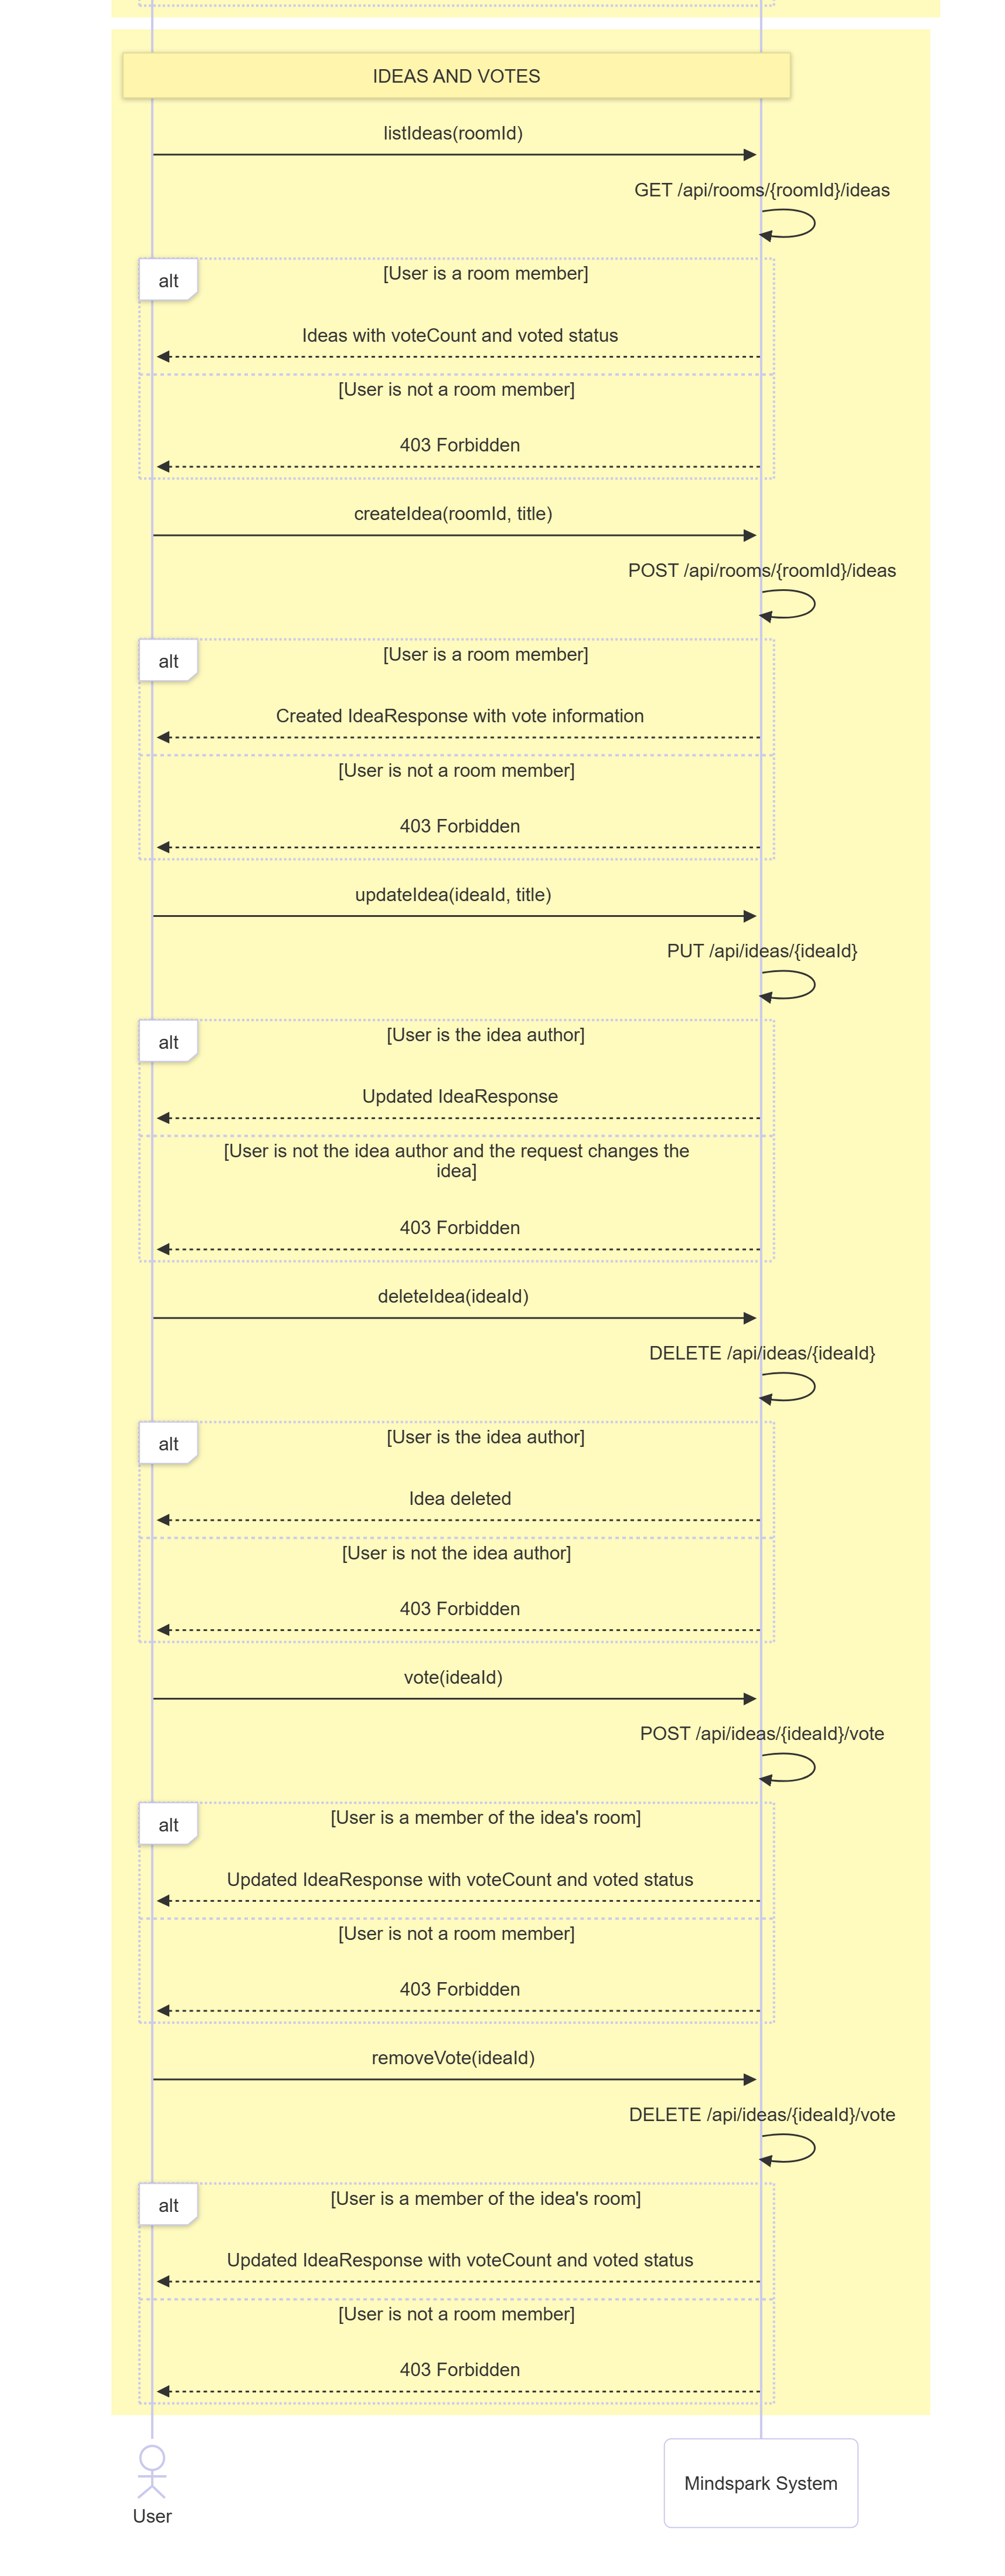
\includegraphics[width=0.95\textwidth,height=0.72\textheight,keepaspectratio]{ideas and vote.png}
    \caption{Idea and vote management sequence diagram}
    \label{fig:sequence-ideas-votes}
\end{figure}

\subsection{Activity Diagram}

The activity diagram illustrates the end-to-end participation flow in a brainstorming session, from authentication to leaving a room. It includes room creation or joining, idea management, and voting. If the room owner leaves, the remaining participants can only leave the room.

\begin{figure}[H]
    \centering
    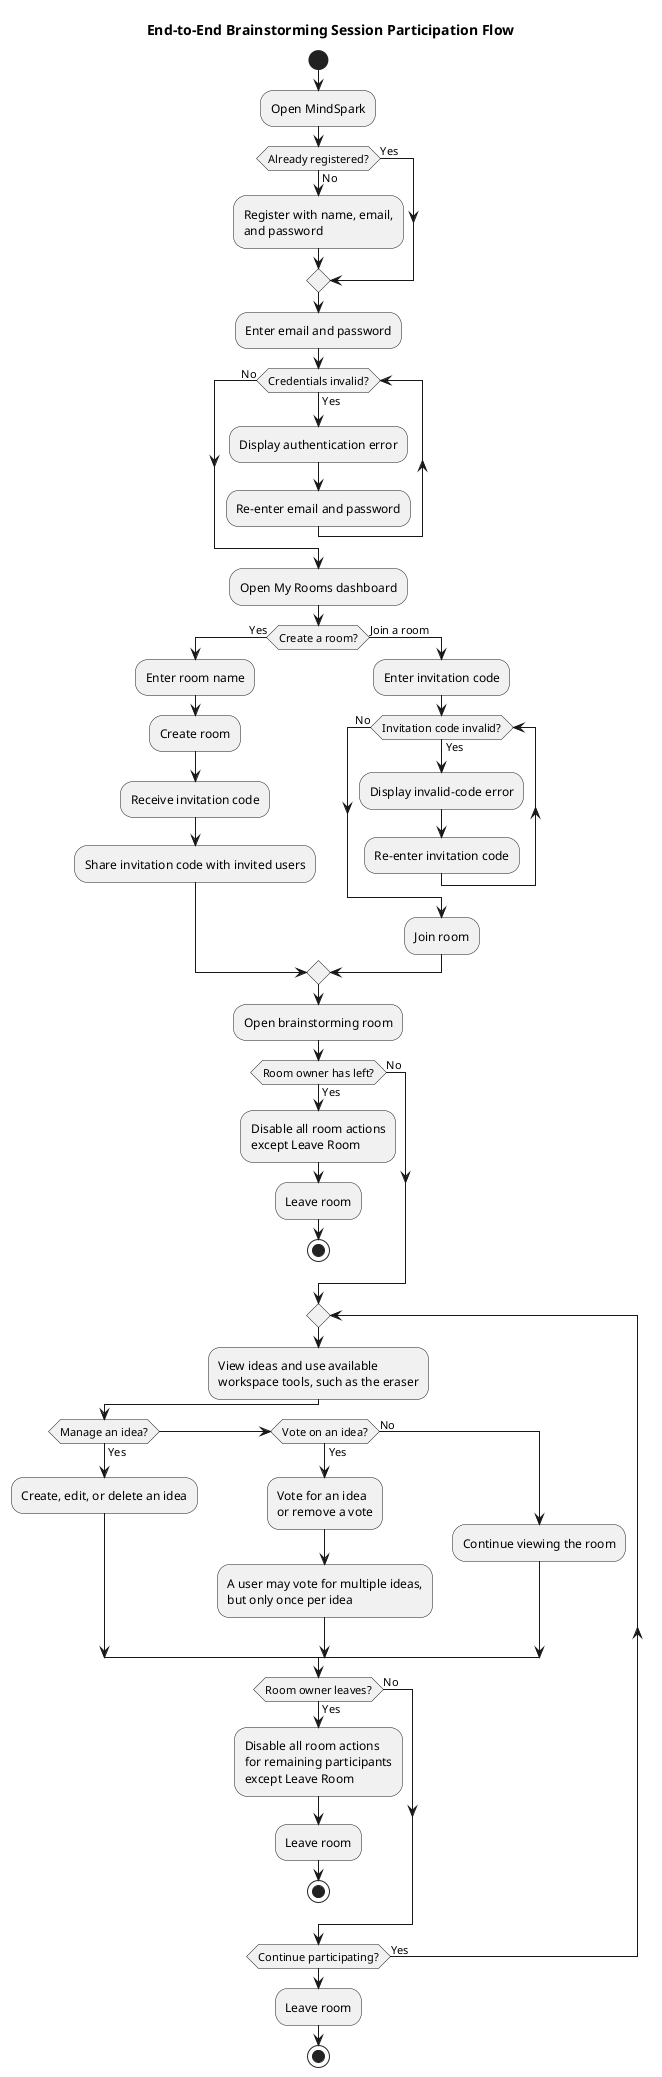
\includegraphics[width=1\textwidth,
        height=0.80\textheight,
        keepaspectratio]{activity_diagram_corrected.png}
    \caption{End-to-end brainstorming session participation flow}
    \label{fig:activity-diagram}
\end{figure}


\section{Implementation Screenshots}
The screenshots below illustrate the main stages of the user experience in MindSpark. They show the account access screens, the My Rooms dashboard, the brainstorming room workspace, and the interface for creating ideas and casting votes. Together, they provide a visual overview of the implemented features discussed in this chapter.



\begin{figure}[H]
    \centering
    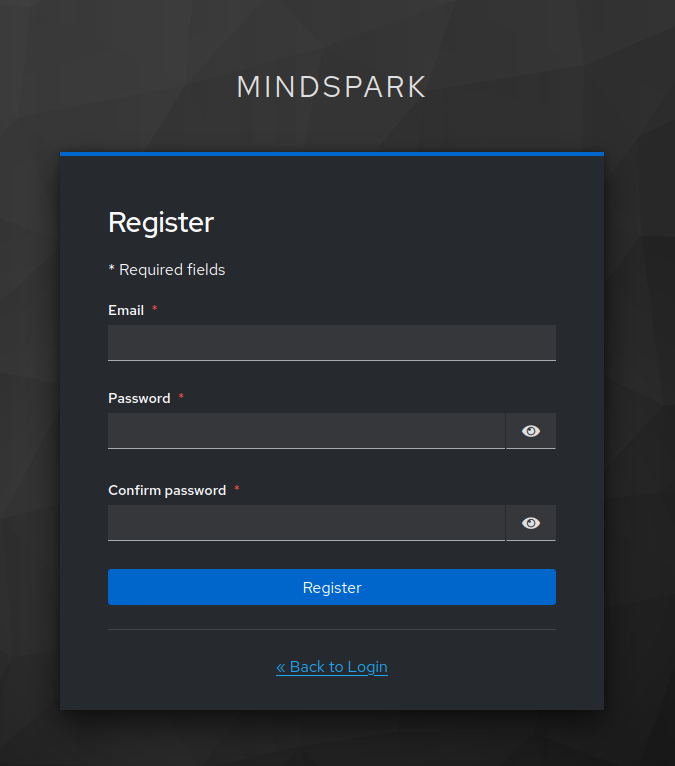
\includegraphics[
        width=0.9\textwidth,
        height=0.6\textheight,
        keepaspectratio
    ]{Keycloak authentification.png}
    \caption{Registration and login screens}
    \label{fig:register-login}
\end{figure}
\screenshotplaceholder{My Rooms dashboard (US-12).}
\begin{figure}[H]
    \centering
    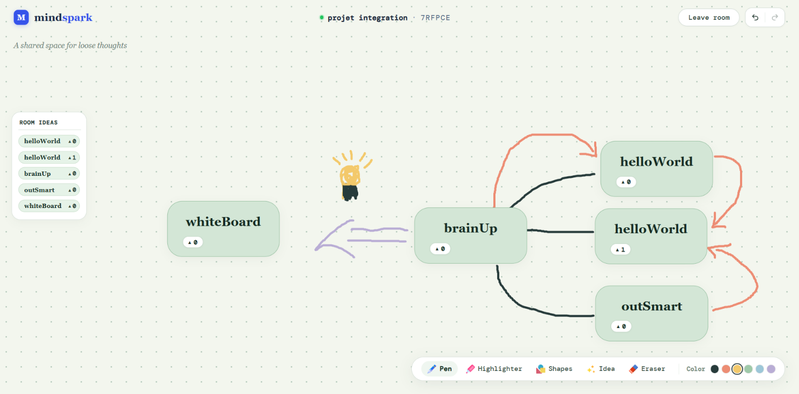
\includegraphics[
        width=0.9\textwidth,
        height=0.6\textheight,
        keepaspectratio
    ]{room-page.png}
    \caption{Registration and login screens}
    \label{fig:register-login}
\end{figure}
\screenshotplaceholder{Idea creation and vote counters (US-22, US-35, US-36).}

\section{Sprint 1 Review and Retrospective}
\subsection{Sprint 1 Review}
According to the sprint report, all 18 backlog items were completed and demonstrated in the public environment: 18 of 18 stories and 58 of 58 story points. The demonstration covered registration, login, room creation, joining by invitation code, idea creation, editing and deletion, and voting. Confirm these completion claims against the team's sprint evidence before final submission.

\begin{table}[H]
\centering
\begin{tabularx}{0.9\textwidth}{|p{0.25\textwidth}|Y|p{0.15\textwidth}|}\hline
\textbf{Area} & \textbf{Stories} & \textbf{Status} \\\hline
Foundations & T1, T2, T3, T4 & Done \\\hline
Authentication & US-1, US-2, US-3, US-4 & Done \\\hline
Rooms & US-9, US-10, US-11, US-12 & Done \\\hline
Ideas and votes & US-22, US-23, US-24, US-25, US-35, US-36 & Done \\\hline
\end{tabularx}
\caption{Sprint 1 review summary}
\end{table}

\subsection{Sprint 1 Retrospective}
Complete this table using the team's actual retrospective answers. Do not retain the prompts as final answers.

\begin{table}[H]
\centering
\begin{tabularx}{\textwidth}{|p{0.30\textwidth}|Y|}\hline
\textbf{Question} & \textbf{Team answer} \\\hline
What went well? & The team completed the planned Sprint 1 backlog and connected the main application components. The registration, room management, idea management, and voting features were integrated into a working demo. \\\hline
 \\\hline
What could be improved? & Some requirements and edge cases could have been clarified earlier, especially permissions when the room owner leaves and handling invalid invitation codes. Testing and integration could also be performed more regularly throughout the sprint. \\\hline
 \\\hline
Actions for Sprint 2 & Define clear acceptance criteria before implementation, review progress regularly, and integrate and test features continuously.  \\\hline
 \\\hline
\end{tabularx}
\caption{Sprint 1 retrospective: team responses to be added}
\end{table}

\clearpage
\section{Conclusion}
Sprint 1 established the foundations for MindSpark and, according to the sprint review, delivered a publicly deployed demo in which a user can register, create or join a room using an invitation code, contribute ideas, and vote. The sprint backlog comprises 18 items and 58 story points.

The system's voting rule allows a user to vote for multiple ideas, while preventing duplicate votes by the same user on the same idea. If the room creator leaves, the remaining participants can no longer perform room actions and may only leave the room. These rules should be reflected consistently in the final diagrams and implementation evidence.

The next sprint can build on these foundations by adding real-time collaboration, online presence, comments, categories, and AI-assisted features, as planned by the team.

\end{document}
